% This file should be compiled as such: PdfLatex -> Bibtex -> PdfLatex (x2)


\documentclass[10pt,a4paper]{article}



\usepackage[utf8]{inputenc}

\usepackage{amsmath}
\newcommand\Rey{\mathrm{Re}}

\usepackage{amsfonts}
\usepackage{amssymb}
\usepackage{outlines}
\usepackage{xcolor}

\usepackage{lineno}
\renewcommand\linenumberfont{\normalfont\small\sffamily}
\linenumbers

\usepackage{graphicx}
\graphicspath{{../pics/}}

\usepackage{natbib}



\author{Jordan Wingenroth, Candace Yee, Justin Nghiem, and Laurel Larsen}



\title{Modeling effective collector efficiency of sparse and dense arrays of cylindrical collectors in varying states of flow velocity and turbulence}



\begin{document}



\maketitle



\paragraph{Editing notes:} 

\textcolor{green!50!red}{Parenthetical insertions in this color are author/editor notes referring to the preceding word or phrase}



\paragraph{Figures:}

I'm aiming for 10-12 figures; 3 methods, 7 results or thereabouts

\begin{itemize}

\item Methods: Direct interception and capture efficiency diagram

\marginpar{Borrrowed from Fauria 2015. We should ask her permission before submitting, correct? Also, if we should make our own or swap in a different figure, let me know.}

\begin{figure}[h]
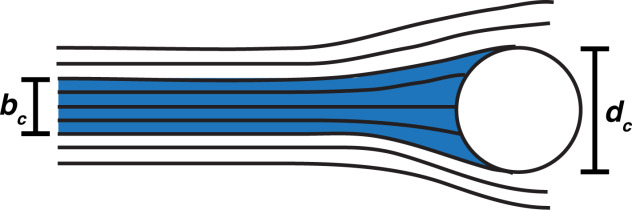
\includegraphics[width=10cm]{fauria particle capture efficiency diagram.jpg}
\centering
\caption{Particle capture efficiency diagram}
\end{figure}

\item Methods: Particle size distribution

\begin{figure}[h]
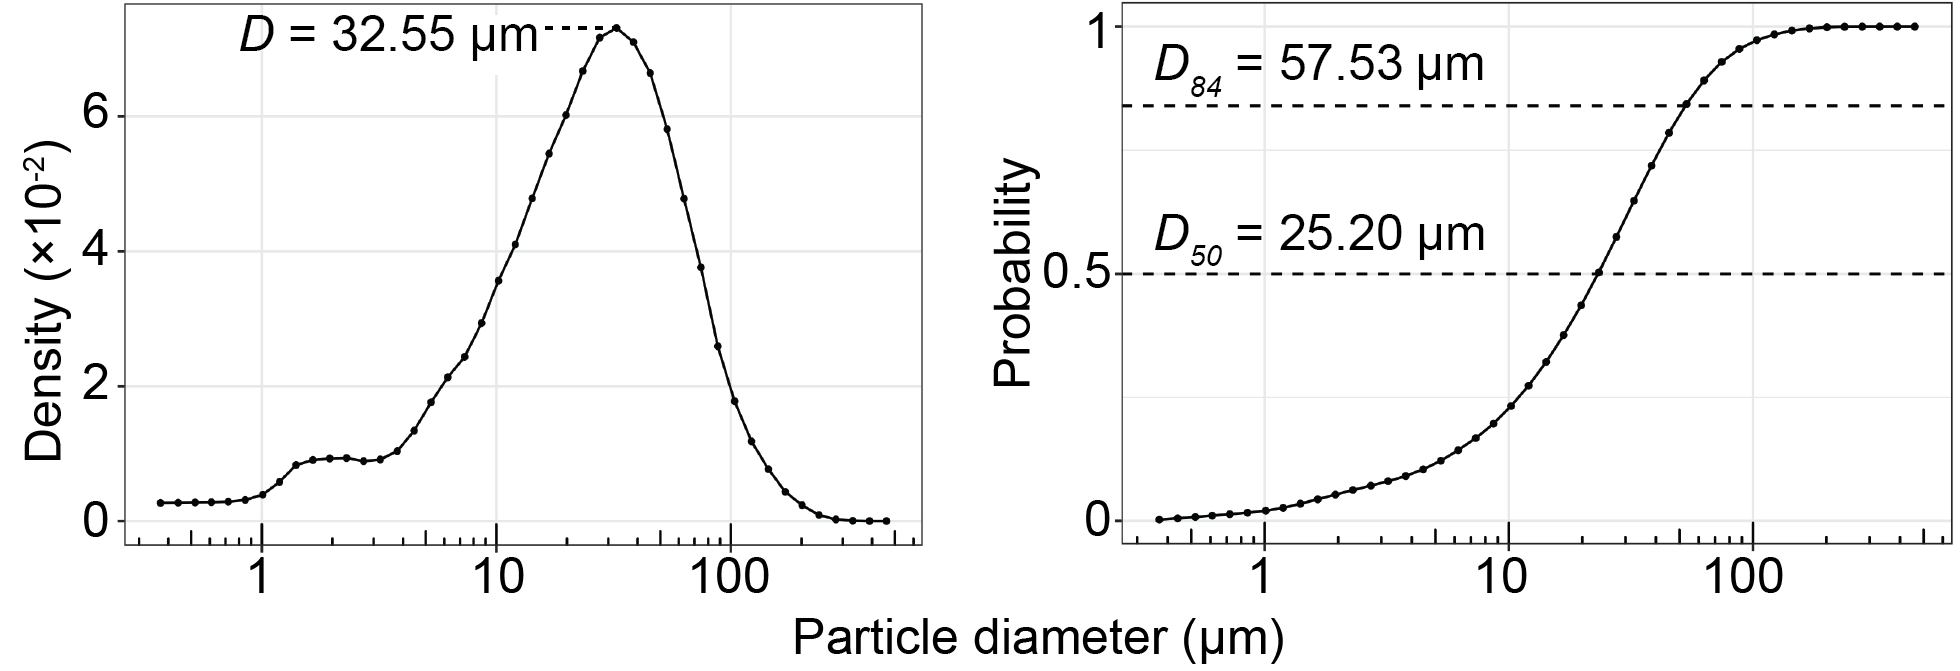
\includegraphics[width=10cm]{wf5-200sizedist.png}
\centering
\caption{Walnut shell particle size distribution}
\end{figure}

\item Methods: Flume floorplan

The figure from the grant proposal has a few features different from the experimental setup. TODO: I'm going to look in the flume manual for a blueprint

\end{itemize}



\section{Introduction}

TODO\\
\hfill\break
Example citation \citep{Fauria_2015}.


\section{Methods}

\subsection{Theoretical Background}

In this study, we focus on direct interception of suspended particles by submerged vegetation. Direct interception is the adhesion of particles traveling along streamlines to the surfaces of collectors (e.g., plants). This is just one of many fluid dynamics mechanisms that act on suspended particles. Others include gravitational settling, inertial impaction, and diffusional deposition. Gravitational settling is the process of particles denser than water being drawn towards and coming to rest on the channel bottom. Inertial impaction and diffusional deposition are other means by which suspended particles can adhere to collectors. Inertial impaction occurs when particles possess momentum relative to streamlines, and diffusional deposition arises due to some combination of turbulence and Brownian motion.

In transitionally turbulent flows ($1 < Re_c < 10^3$), which 



\subsection{Suspended Particle Concentration Model}
\marginpar{Note: Same subsection title as Fauria 2015. Should we change? Any ideas?}

$$\frac{d\bar{\phi}}{dt} = -[\frac{Cv_s}{h}(1-E_r) + \eta^{\prime}ud_cI_c]\bar{\phi} = -k\bar{\phi}$$

\subsection{Experimental Methods}
\marginpar{Note: Same subsection title as Fauria 2015. Should we change? Any ideas?}



\subsubsection{Materials}

Our experiment was conducted in a recirculating flume. Water was propelled by an electric pump through a rectangular pipe of gradually increasing hydraulic diameter (intended to avoid abrupt changes in velocity), through a honeycomb flow collimator, into a rectangular open channel containing our test section, then through another similar pipe feeding back to the pump (Figure XY). In the upper range of the pump's span, cavitation (i.e., taking on air bubbles) occured, which was accompanied by a distinct noise. By gradually increasing the pump's velocity while monitoring for sound, we determined that the pump chambers stayed free of cavitation up to a rotation speed well above 30 Hz, which was chosen as the maximum velocity for our experimental treatments.

We installed collectors in a removable array which was installed to fill a recessed well in the bottom of the rectangular channel. The perforated top of the array gaps between the array and the upstream and downstream edges of the well were covered with flat, rectangular pieces of aluminum secured with 

\subsubsection{Particle Concentration Run Protocols}



\subsubsection{Flow Characterization Run Protocols}



\subsection{Statistical Analysis}



\section{Results}

TODO



\section{Discussion}

TODO\\
\hfill\break
The assumption that probability of retention ($p_r$) is 100\% when stems are coated with grease might be questionable based on our result that biofilm increased $\eta\prime$. The only other effect of biofilm that is readily apparent to me is perhaps increasing effective stem diameter ($d_c$). However, with our model for Reynolds number ($\Rey_c \propto d_c$), and both us and \citet{Fauria_2015} finding $\eta\prime \sim -\Rey_c$, increasing stem diameter would be expected to have the opposite effect, unless I'm missing something.



\bibliographystyle{apalike}
\bibliography{refs}



\end{document}

